% =========================================================
% APÉNDICE A — Sensibilidad Paramétrica y Controles de Robustez
% =========================================================

\chapter{Sensibilidad Paramétrica y Controles de Robustez}
\label{ap:sensibilidad}

Este apéndice complementa los resultados del Capítulo~\ref{cap:resultados} con
figuras adicionales que validan la robustez del mecanismo de \emph{Pebble Snow}
frente a variaciones en los parámetros de control. Las figuras aquí presentadas
no forman parte de la narrativa central, pero constituyen la evidencia empírica
que respalda las conclusiones del texto principal.

% ---------------------------------------------------------
\section{Impacto de $v_{\rm frag}$ sobre la Retención Aerodinámica}
% ---------------------------------------------------------

Las Figuras~\ref{fig:ap_hovmoller_v1} y~\ref{fig:ap_hovmoller_v3} presentan los
diagramas de Hovmöller equivalentes a la Figura~\ref{fig:hovmoller} pero para los
casos de control con $v_{\rm frag} = 1\text{ m/s}$ y $v_{\rm frag} = 3\text{ m/s}$
respectivamente.

\begin{figure}[htpb]
    \centering
    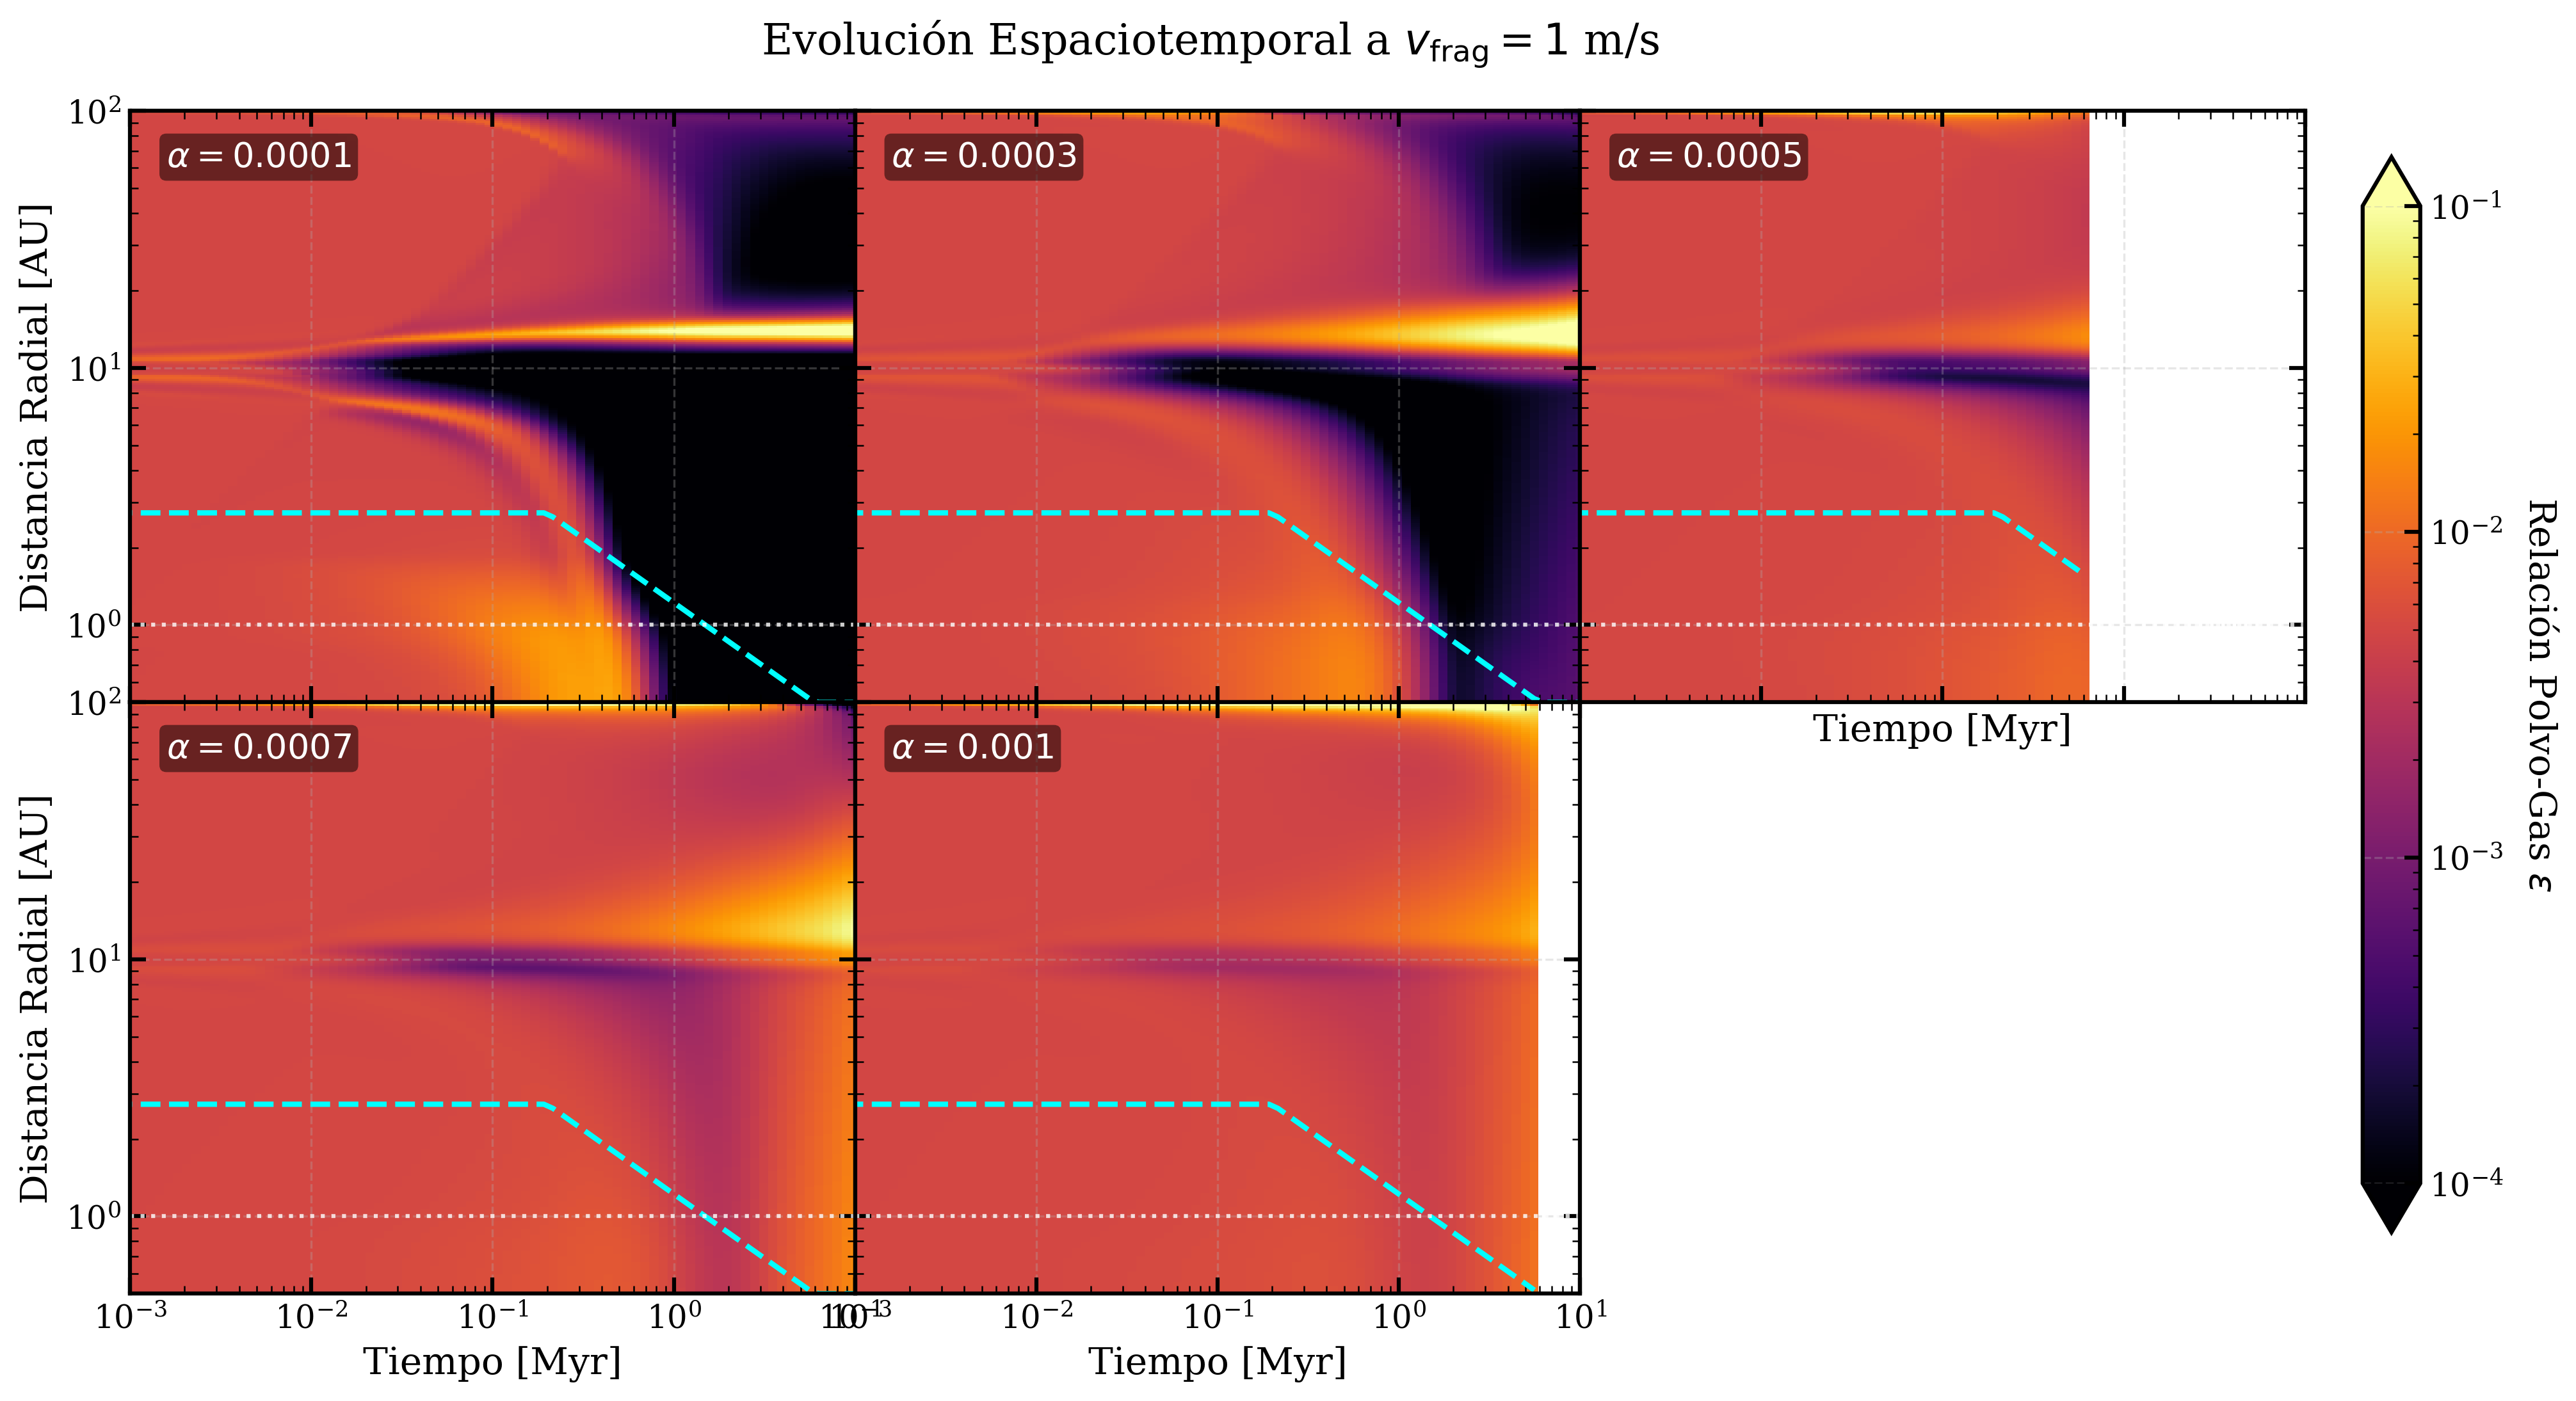
\includegraphics[width=\textwidth]{figures/apendice/hovmoller_v1.png}
    \caption{Diagrama de Hovmöller para $v_{\rm frag} = 1\text{ m/s}$ uniforme.
    La ausencia de diferencial de fragmentación elimina el evento de flushing:
    el anillo de polvo en el gap persiste estáticamente sin liberarse hacia
    el disco interior al ser cruzado por la isoterma de sublimación.}
    \label{fig:ap_hovmoller_v1}
\end{figure}

\begin{figure}[htpb]
    \centering
    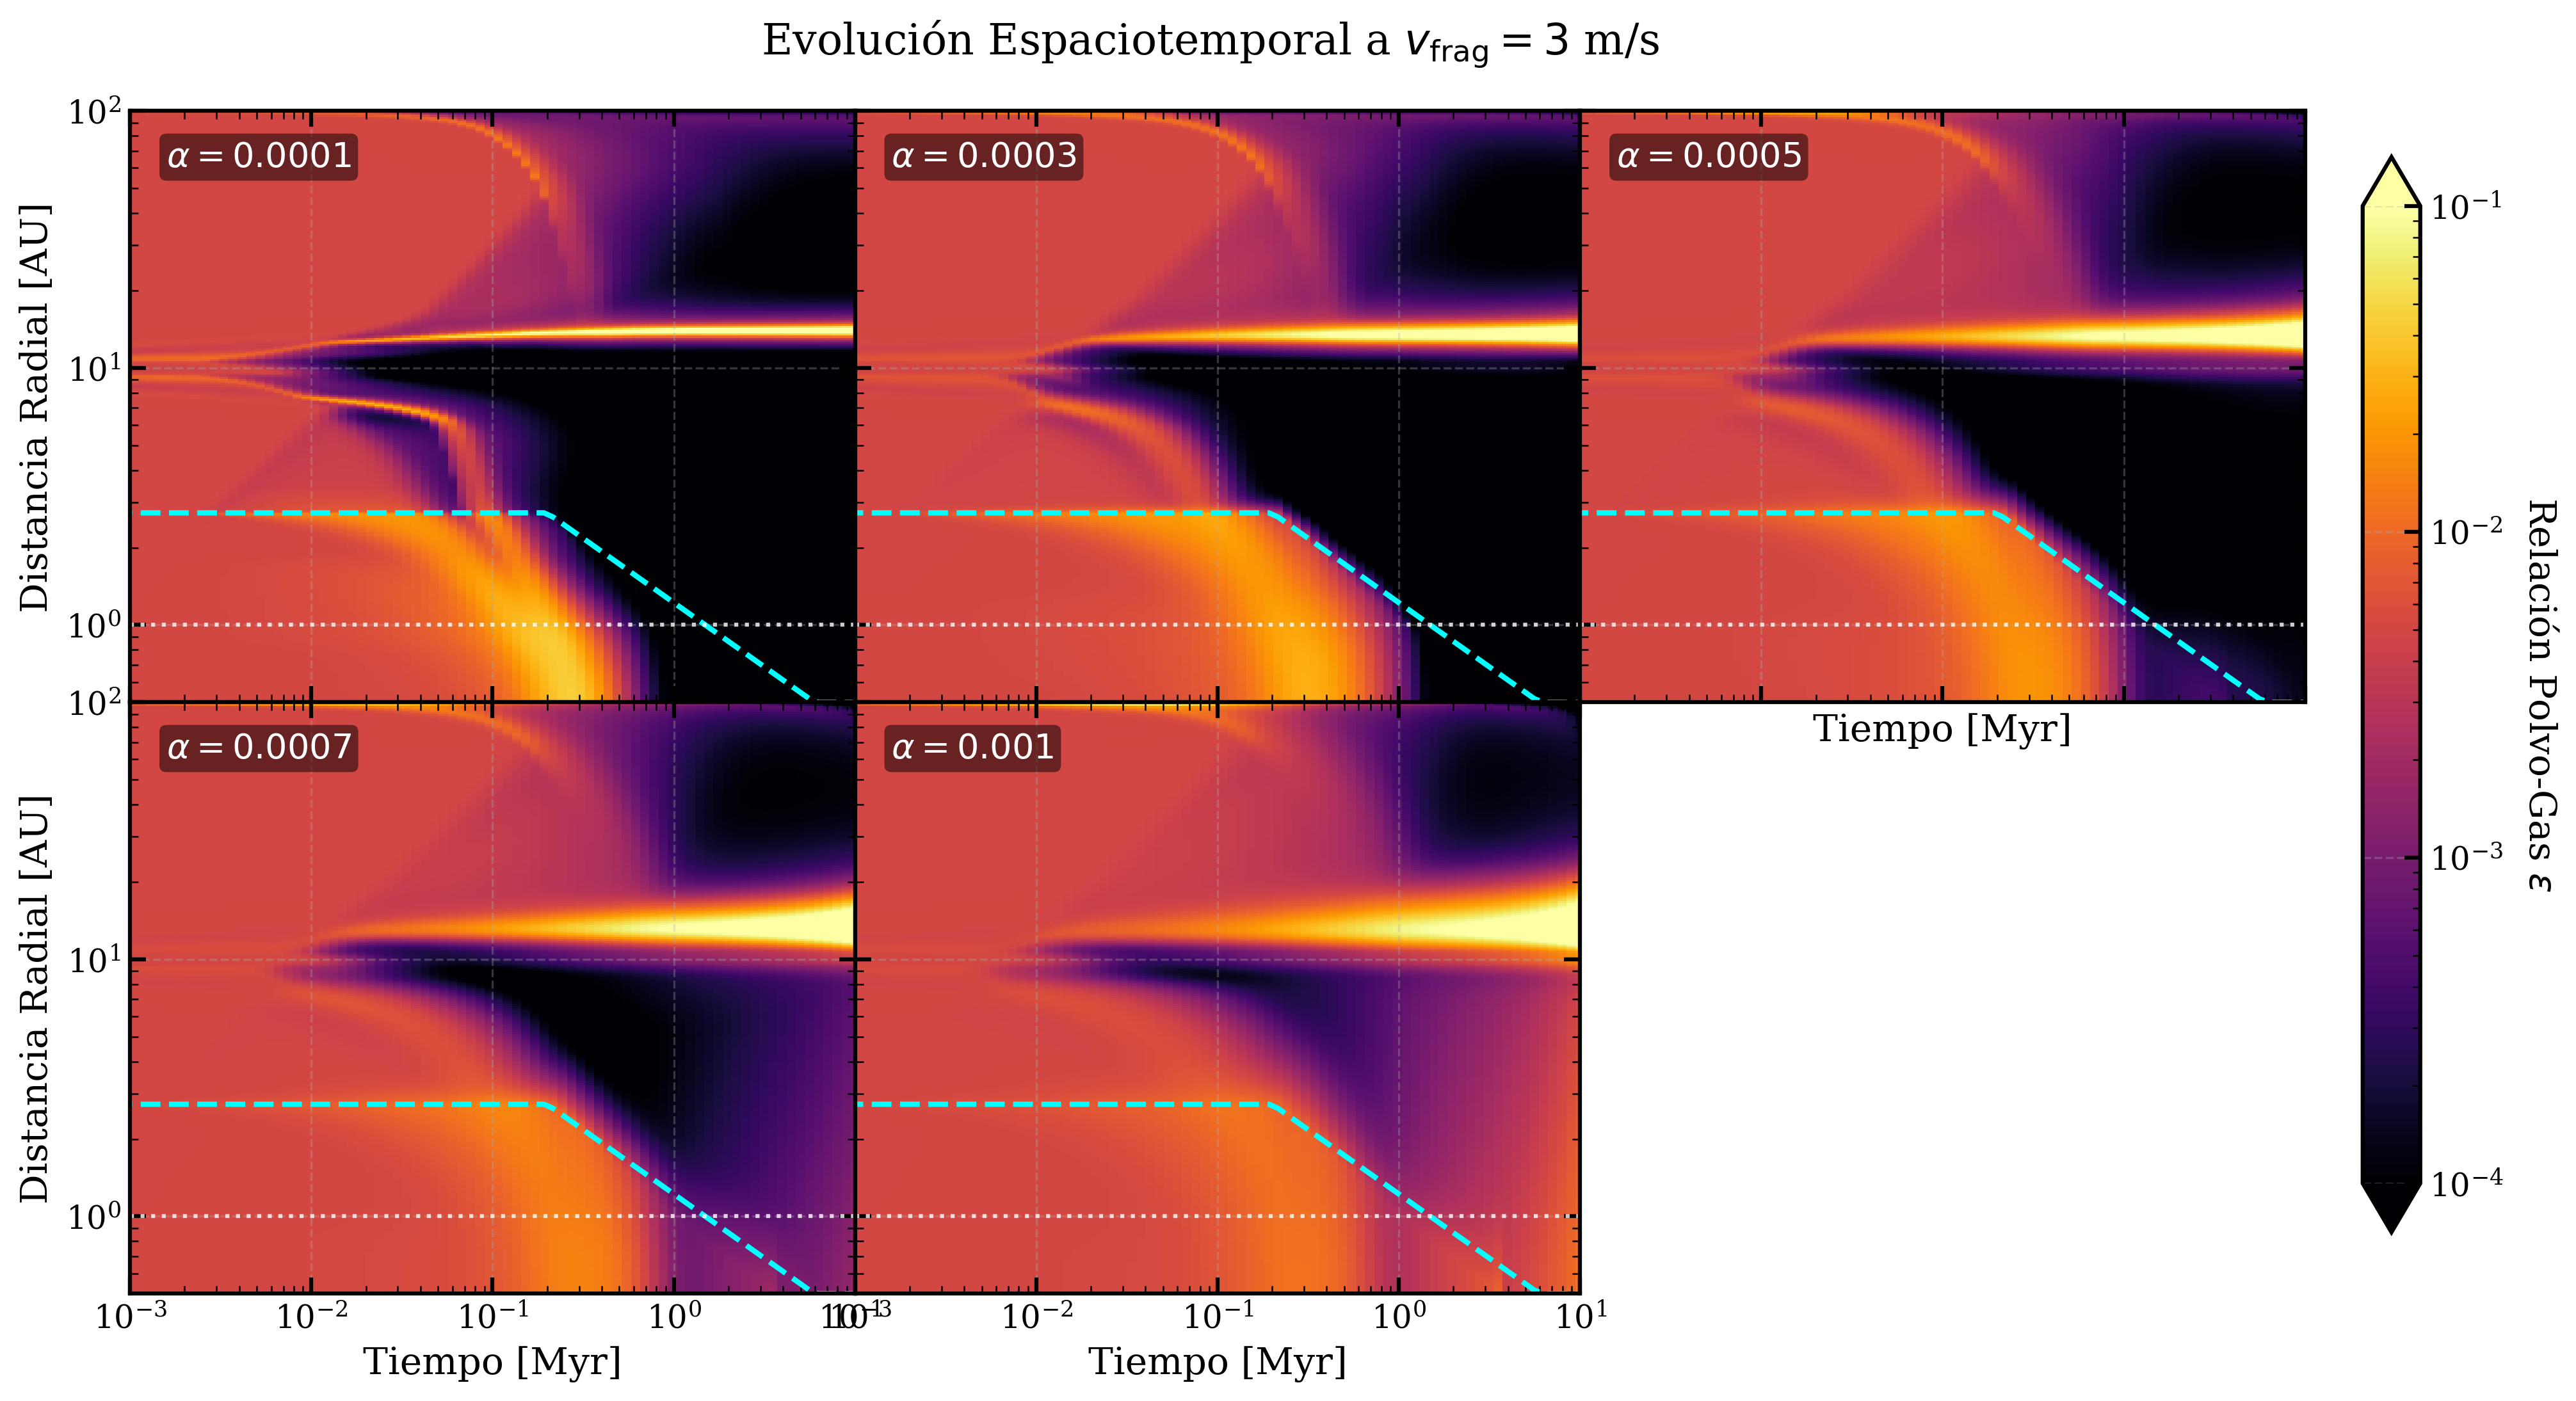
\includegraphics[width=\textwidth]{figures/apendice/hovmoller_v3.png}
    \caption{Diagrama de Hovmöller para $v_{\rm frag}^{\rm ice} = 3\text{ m/s}$.
    Se observa un flushing parcial: el diferencial reducido (factor 3 vs.\ el
    factor 10 del caso canónico) libera una fracción del material retenido al
    cruzar la snowline, produciendo un evento de acreción de menor magnitud
    que en el caso canónico.}
    \label{fig:ap_hovmoller_v3}
\end{figure}

\begin{figure}[htpb]
    \centering
    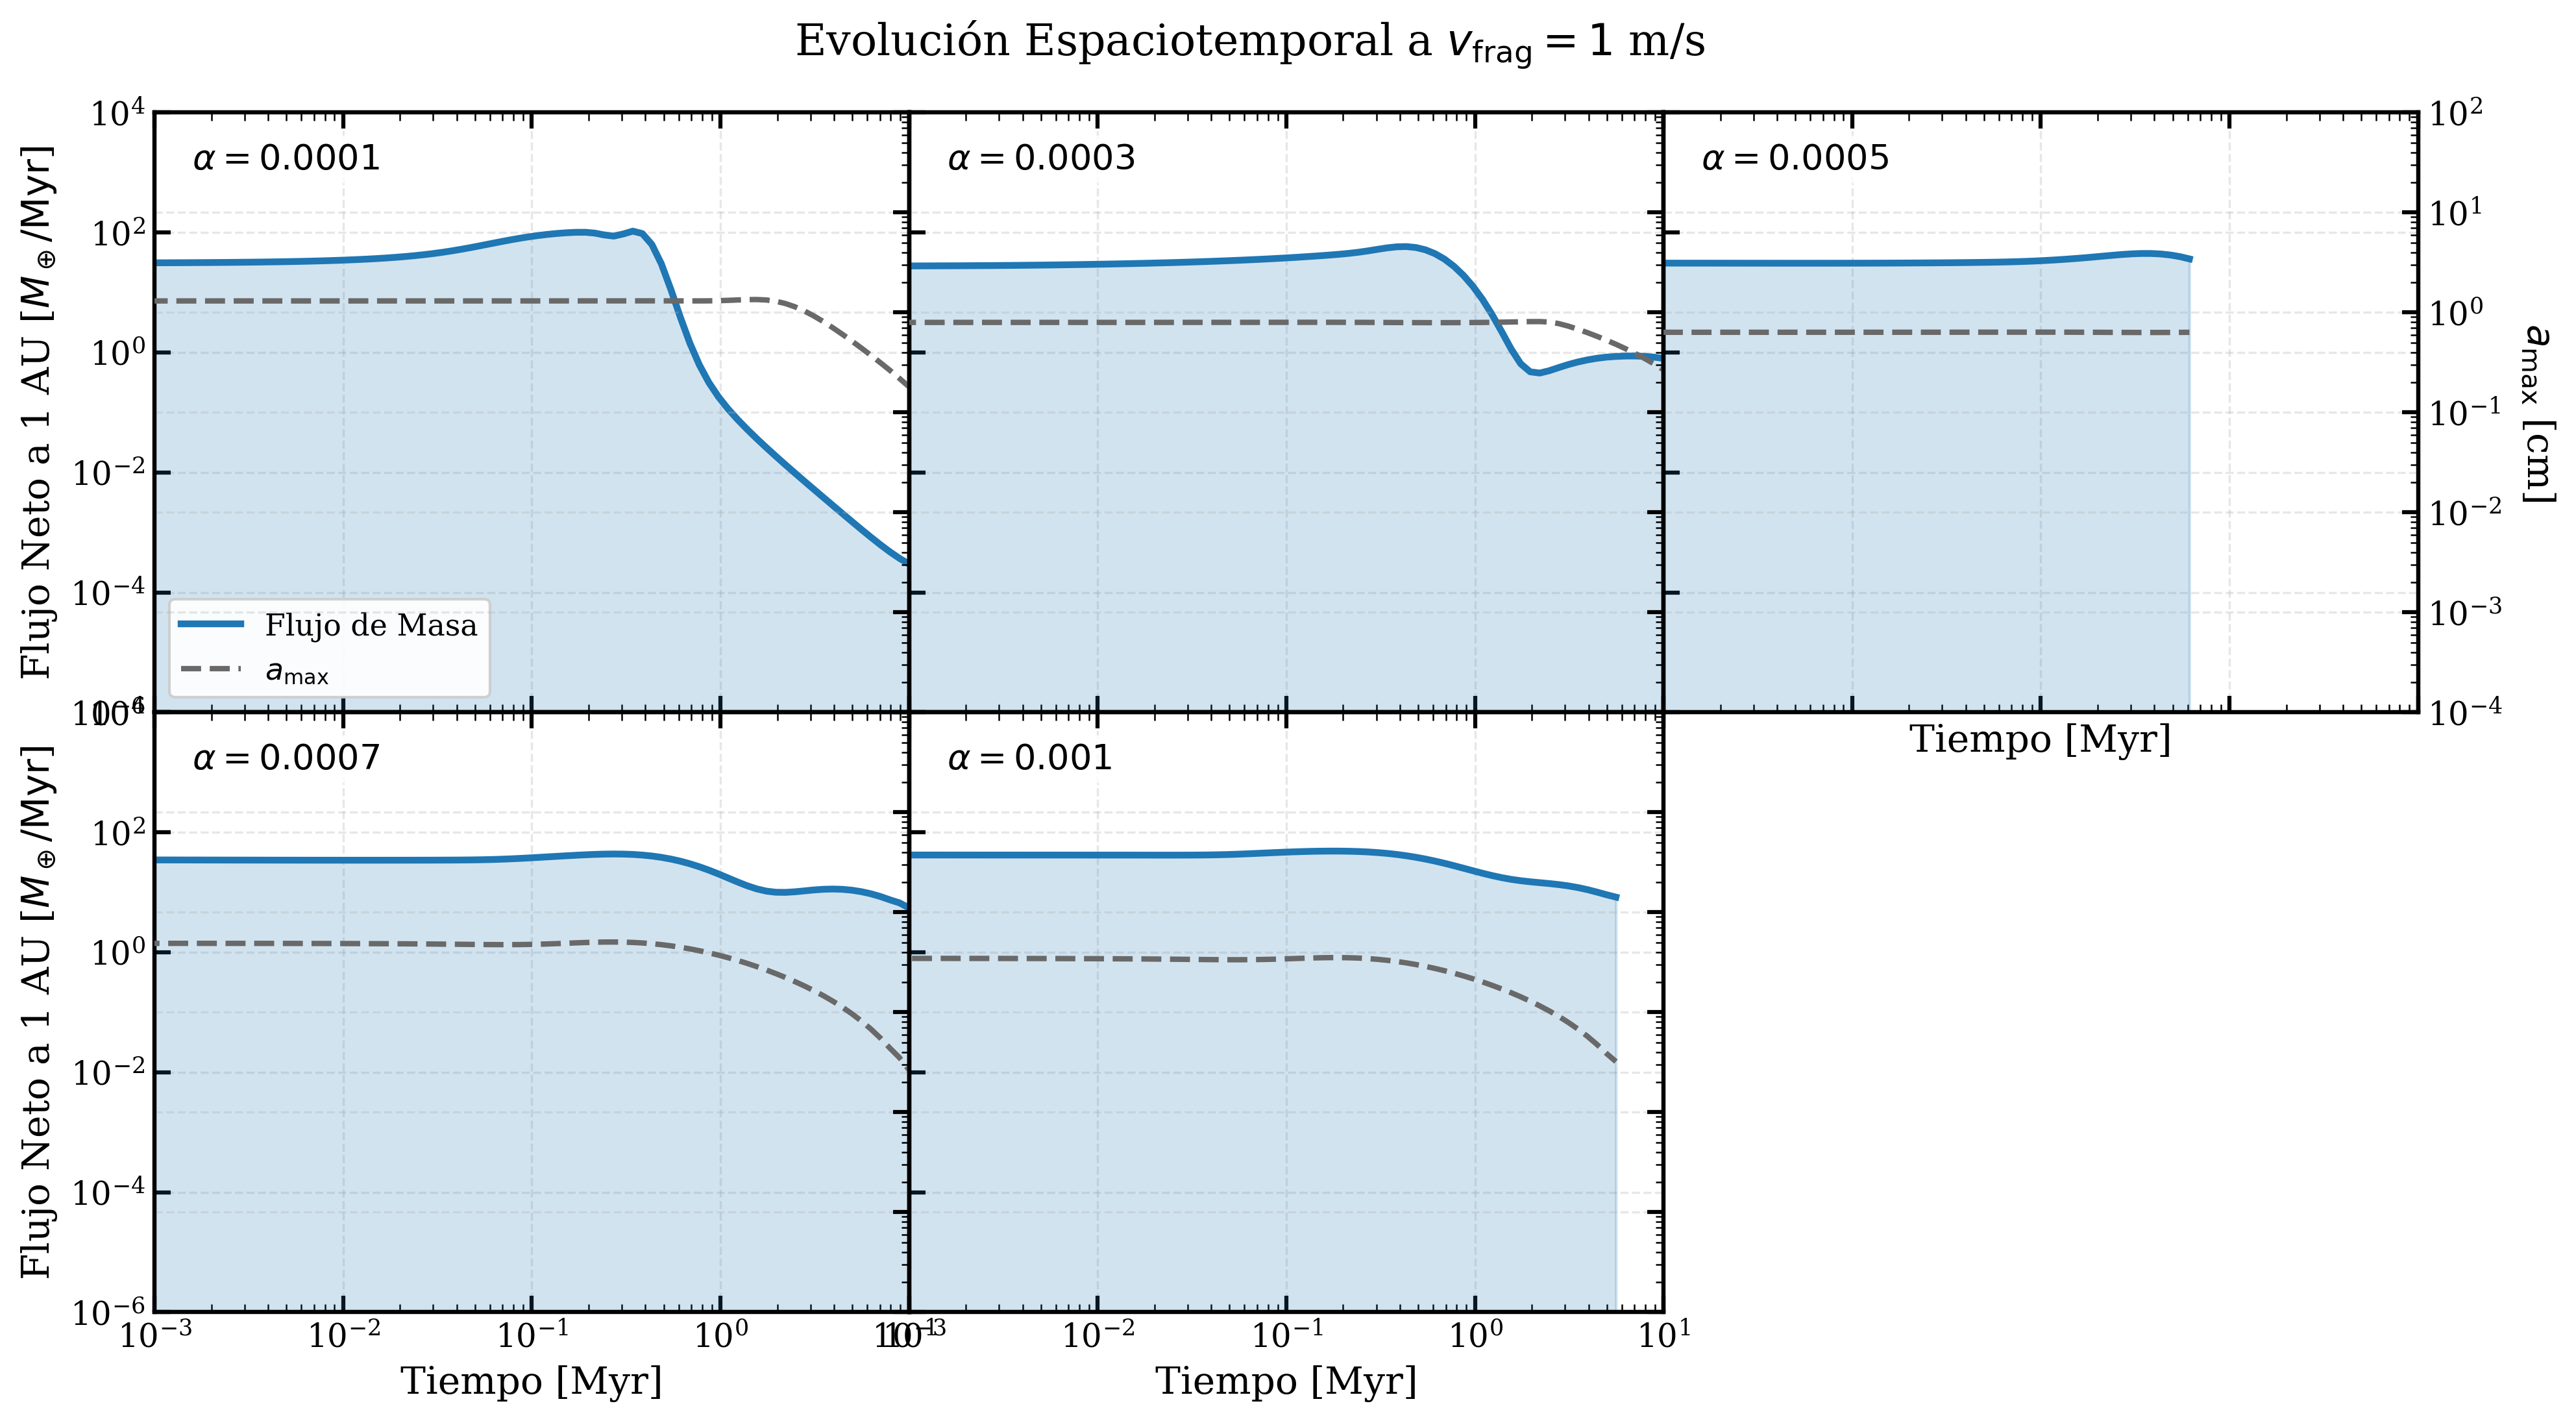
\includegraphics[width=0.49\textwidth]{figures/apendice/flux_amax_v1.png}
    \hfill
    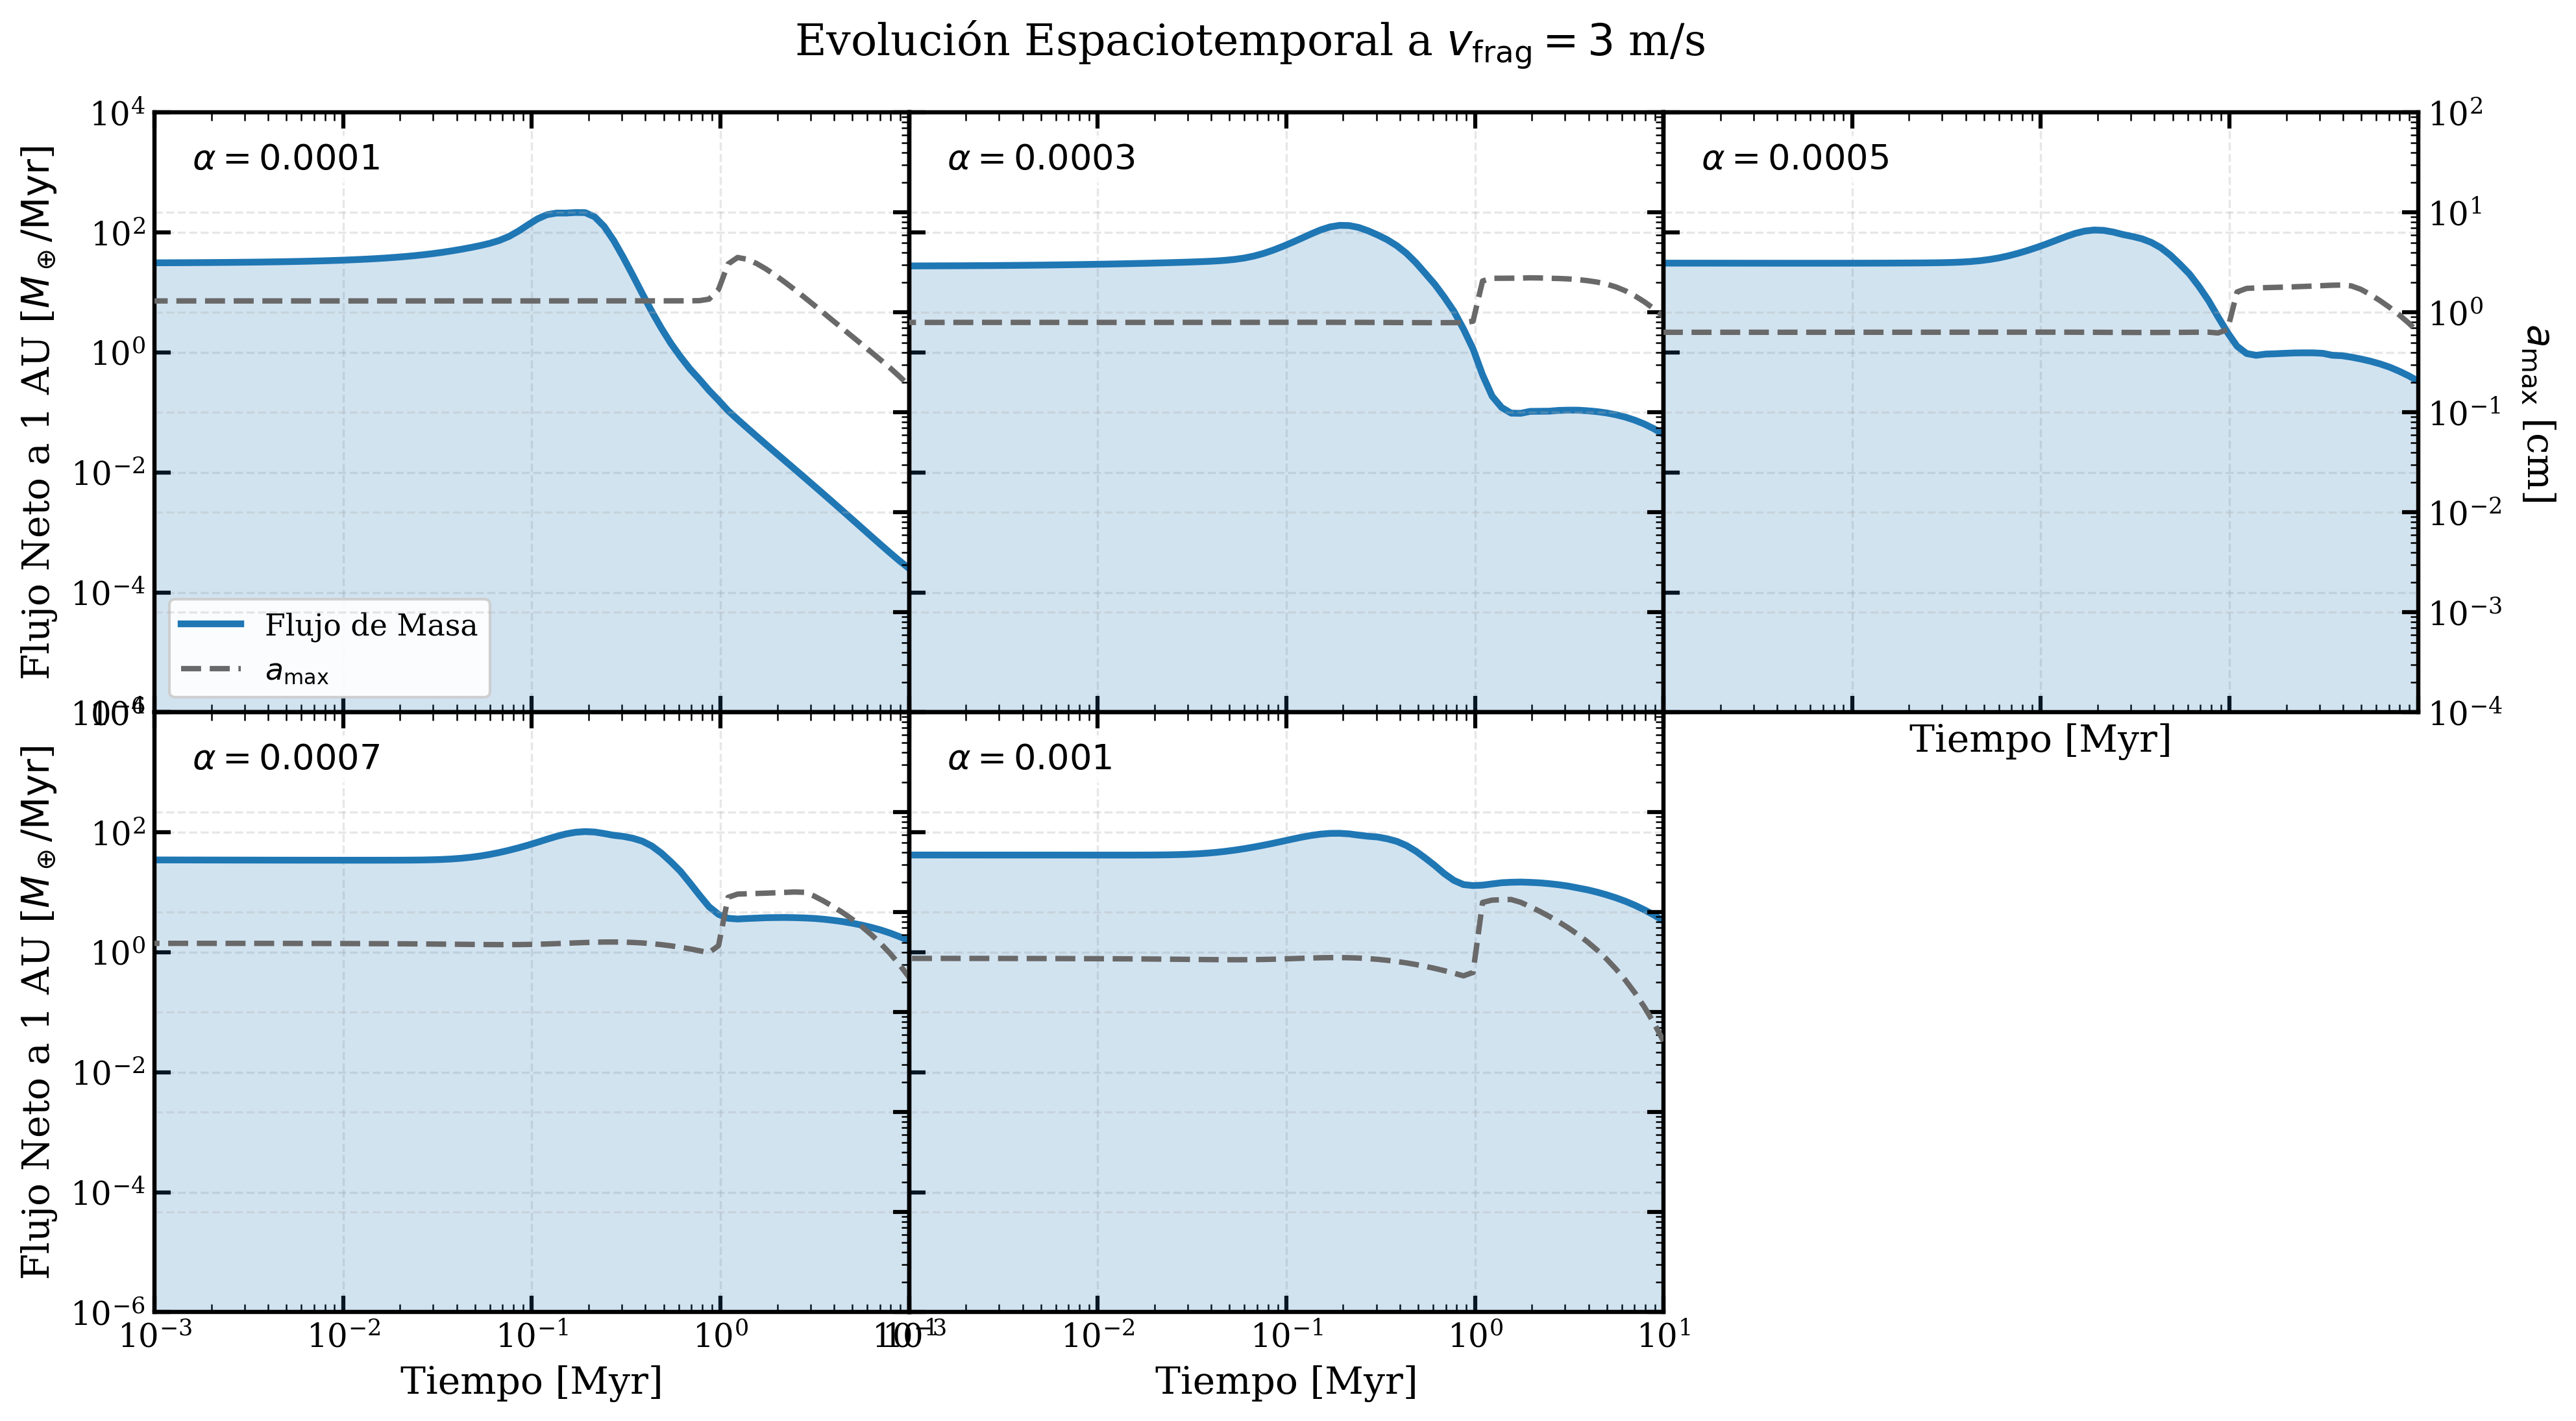
\includegraphics[width=0.49\textwidth]{figures/apendice/flux_amax_v3.png}
    \caption{Perfiles de flujo de pebbles $\dot{M}_{\rm peb}$ y tamaño máximo de
    grano $a_{\rm max}$ para $v_{\rm frag} = 1\text{ m/s}$ (izquierda) y
    $v_{\rm frag} = 3\text{ m/s}$ (derecha). En el caso de 1 m/s, el número de
    Stokes se mantiene continuo al cruzar la isoterma; en el de 3 m/s, la caída
    es moderada pero suficiente para liberar parcialmente el material del gap.}
    \label{fig:ap_flux_amax}
\end{figure}

% ---------------------------------------------------------
\section{Heatmaps del Caso Canónico ($\alpha = 0.001$)}
% ---------------------------------------------------------

Las Figuras~\ref{fig:ap_heatmap_masa} y~\ref{fig:ap_heatmap_h2o} presentan los
heatmaps de masa final y fracción de agua para el caso canónico bien definido
($\alpha = 0.001$, $v_{\rm frag} = 10\text{ m/s}$, $M_0 = 10^{-4}\,M_\oplus$),
mostrando la "Isla de Crecimiento" con mayor resolución que el diagrama de burbujas
de la Figura~\ref{fig:bubble_v10}.

\begin{figure}[htpb]
    \centering
    
\includegraphics[width=0.49\textwidth]{figures/apendice/heatmap_masa.png}
    \hfill
    
\includegraphics[width=0.49\textwidth]{figures/apendice/heatmap_h2o.png}
    \caption{\textit{Izquierda:} Heatmap de masa final $\log(M_c/M_\oplus)$ en
    función de la posición $r_{\rm gap}$ (eje X) y la masa $M_{\rm gap}$ (eje Y)
    del gap planetario.
    \textit{Derecha:} Heatmap de la fracción de agua $f_{\rm H_2O}$ para los
    mismos parámetros.
    La banda de crecimiento exitoso ($M_{\rm gap} \sim 0.1\,M_{\rm Jup}$) es
    claramente visible, así como la correlación entre alta masa final y baja
    fracción de agua en el régimen de filtrado óptimo.}
    \label{fig:ap_heatmap_masa}
    \label{fig:ap_heatmap_h2o}
\end{figure}

% ---------------------------------------------------------
\section{Cronología del Gap: Gaps Retrasados}
% ---------------------------------------------------------

\begin{figure}[htpb]
    \centering
    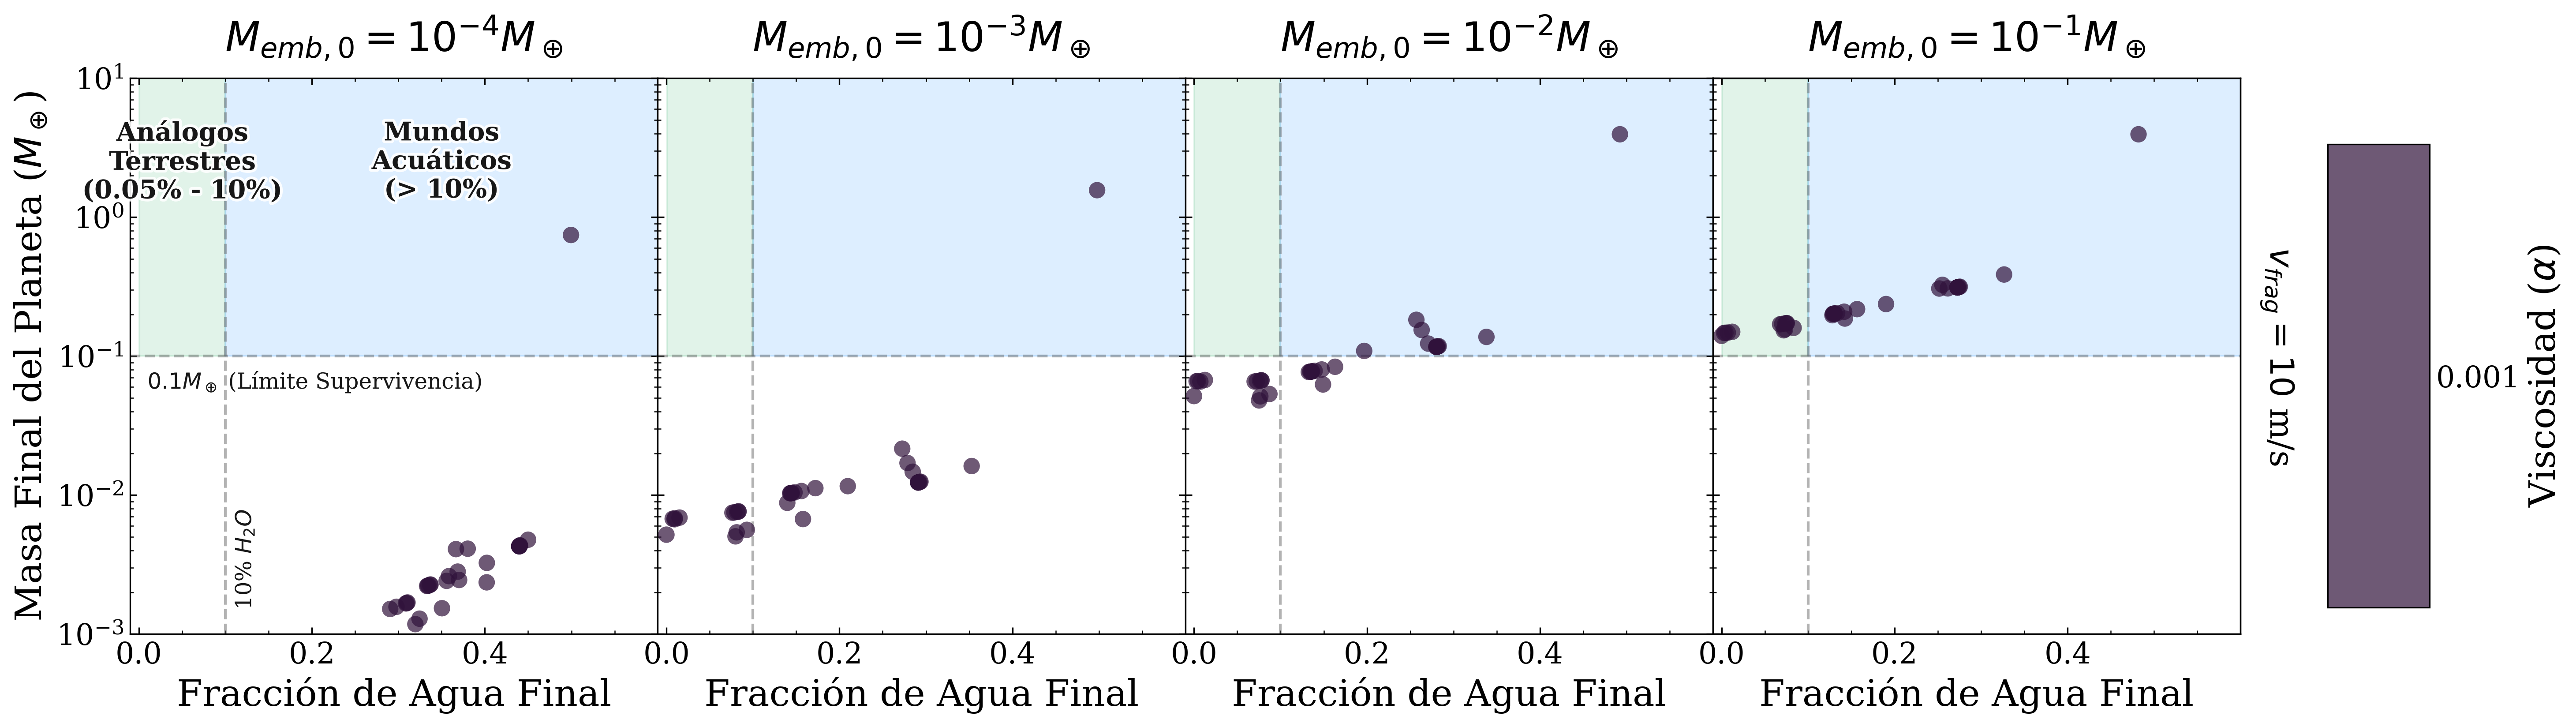
\includegraphics[width=\textwidth]{figures/apendice/population_delayed.png}
    \caption{Curvas de crecimiento del embrión para distintos tiempos de inserción
    del gap $t_{\rm gap}$ (colores). El gap se ubica a 10 AU con
    $M_{\rm gap} = 0.1\,M_{\rm Jup}$ y $\alpha = 0.001$.
    Para $t_{\rm gap} \ge 2\text{ Myr}$, la mayor parte del inventario sólido
    primordial ya ha derivado hacia la estrella antes de que el gap se forme,
    eliminando el reservorio de material disponible para el evento de flushing.}
    \label{fig:ap_delayed}
\end{figure}

% ---------------------------------------------------------
\section{Distribución Volumétrica en Discos Sinusoidales}
% ---------------------------------------------------------

\begin{figure}[htpb]
    \centering
    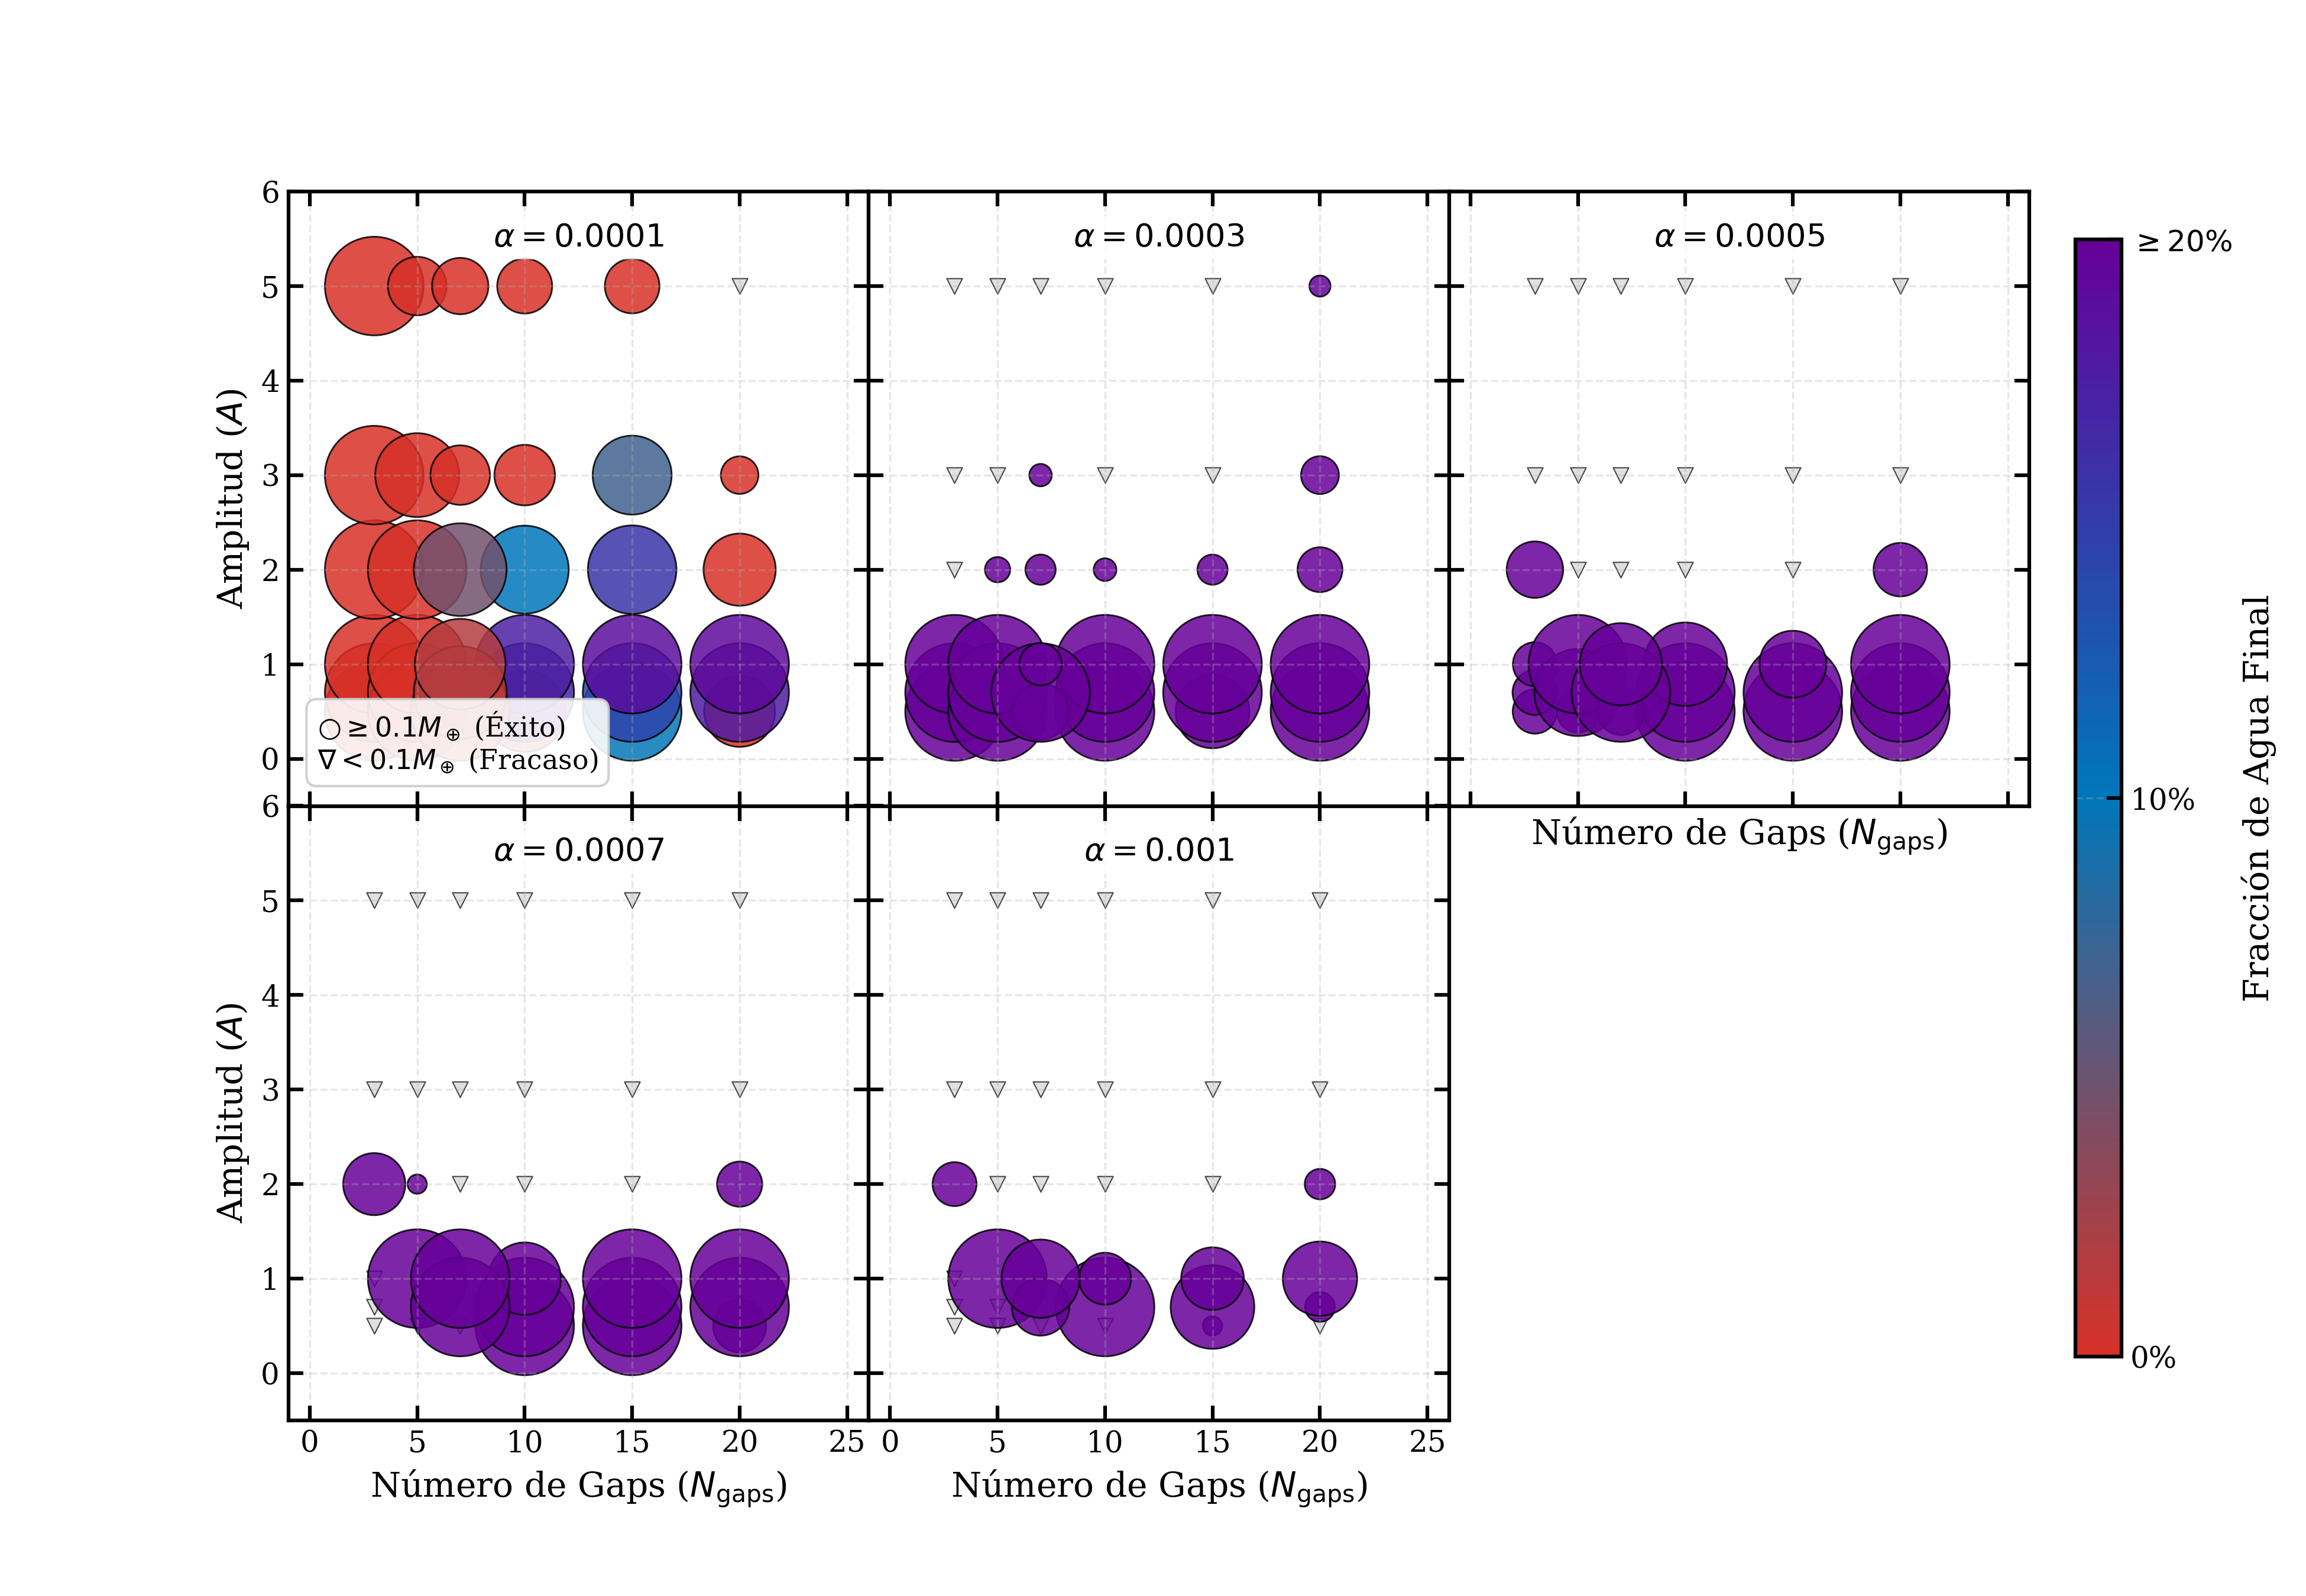
\includegraphics[width=\textwidth]{figures/apendice/bubble_sinusoidal_v10.png}
    \caption{Diagrama de burbujas para configuraciones sinusoidales con
    $v_{\rm frag} = 10\text{ m/s}$. El diámetro de cada punto es proporcional
    a $M_c$; el color indica $f_{\rm H_2O}$. La ausencia de burbujas grandes
    en el régimen de alta amplitud ($A \ge 3.0$) confirma que las subestructuras
    periódicas profundas suprimen la formación de embriones masivos en las
    regiones interiores del disco.}
    \label{fig:ap_bubble_sin}
\end{figure}

% ---------------------------------------------------------
\section{Validación Numérica: Sensibilidad a $M_{\rm cross}$}
% ---------------------------------------------------------

Para verificar que los resultados no son artefactos de la parametrización específica
de la migración de la isoterma, se repitieron simulaciones variando el parámetro
$M_{\rm cross}$, que controla el tiempo de cruce de la snowline en el modelo de
Oka \& Hartmann. Las Figuras~\ref{fig:ap_mcross_masa} y~\ref{fig:ap_mcross_h2o}
muestran que la masa final y la fracción de agua son insensibles a variaciones de
$M_{\rm cross}$ dentro de rangos físicamente plausibles, confirmando la universalidad
del mecanismo.

\begin{figure}[htpb]
    \centering
    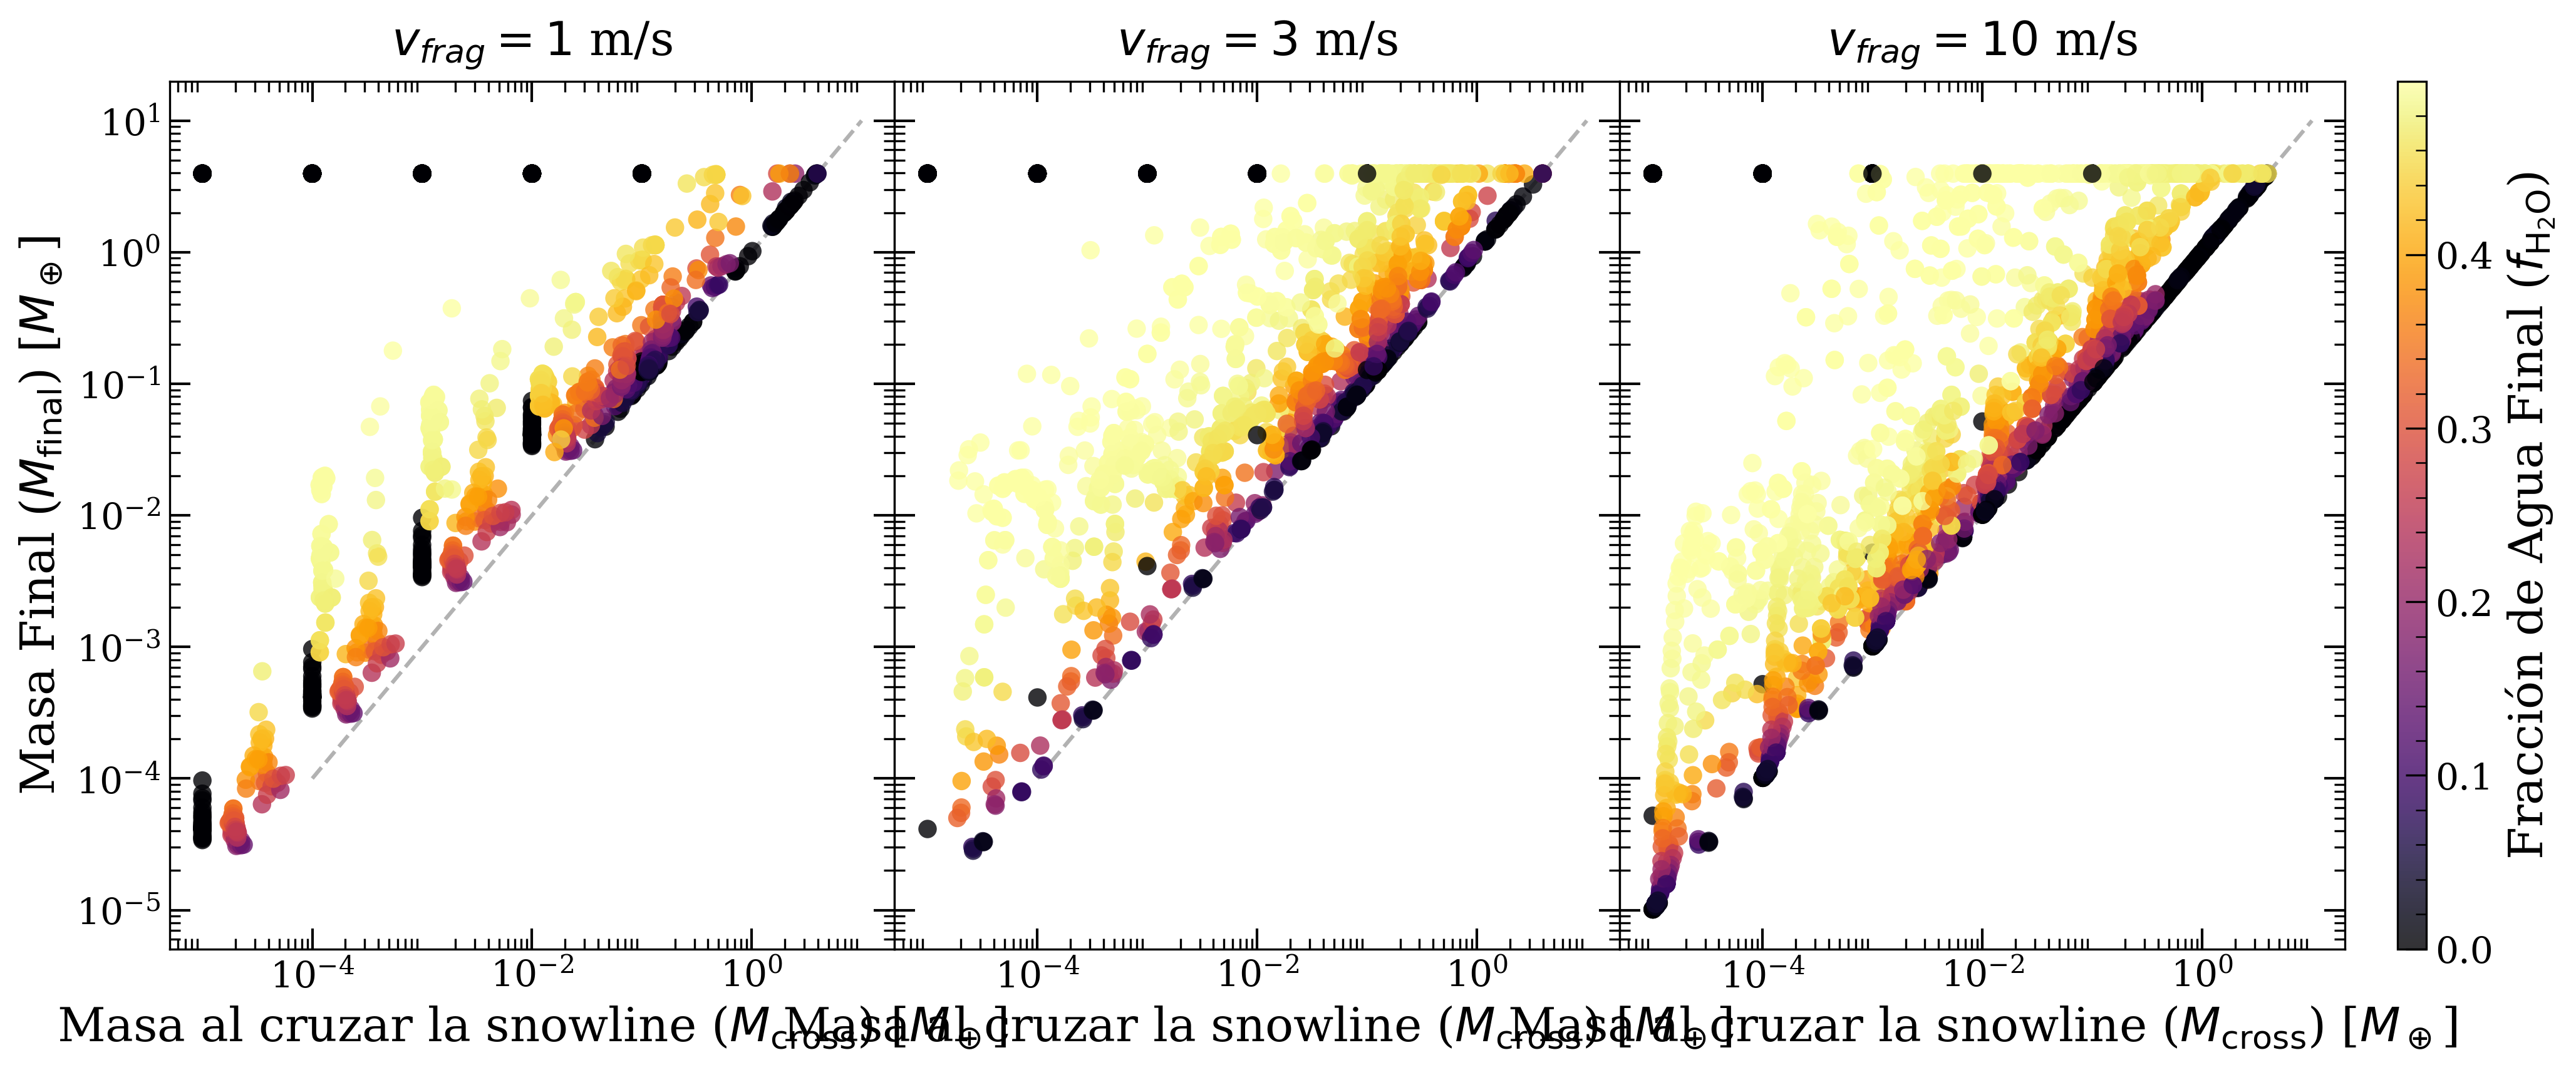
\includegraphics[width=0.49\textwidth]{figures/apendice/FigC_Mcross.png}
    \hfill
    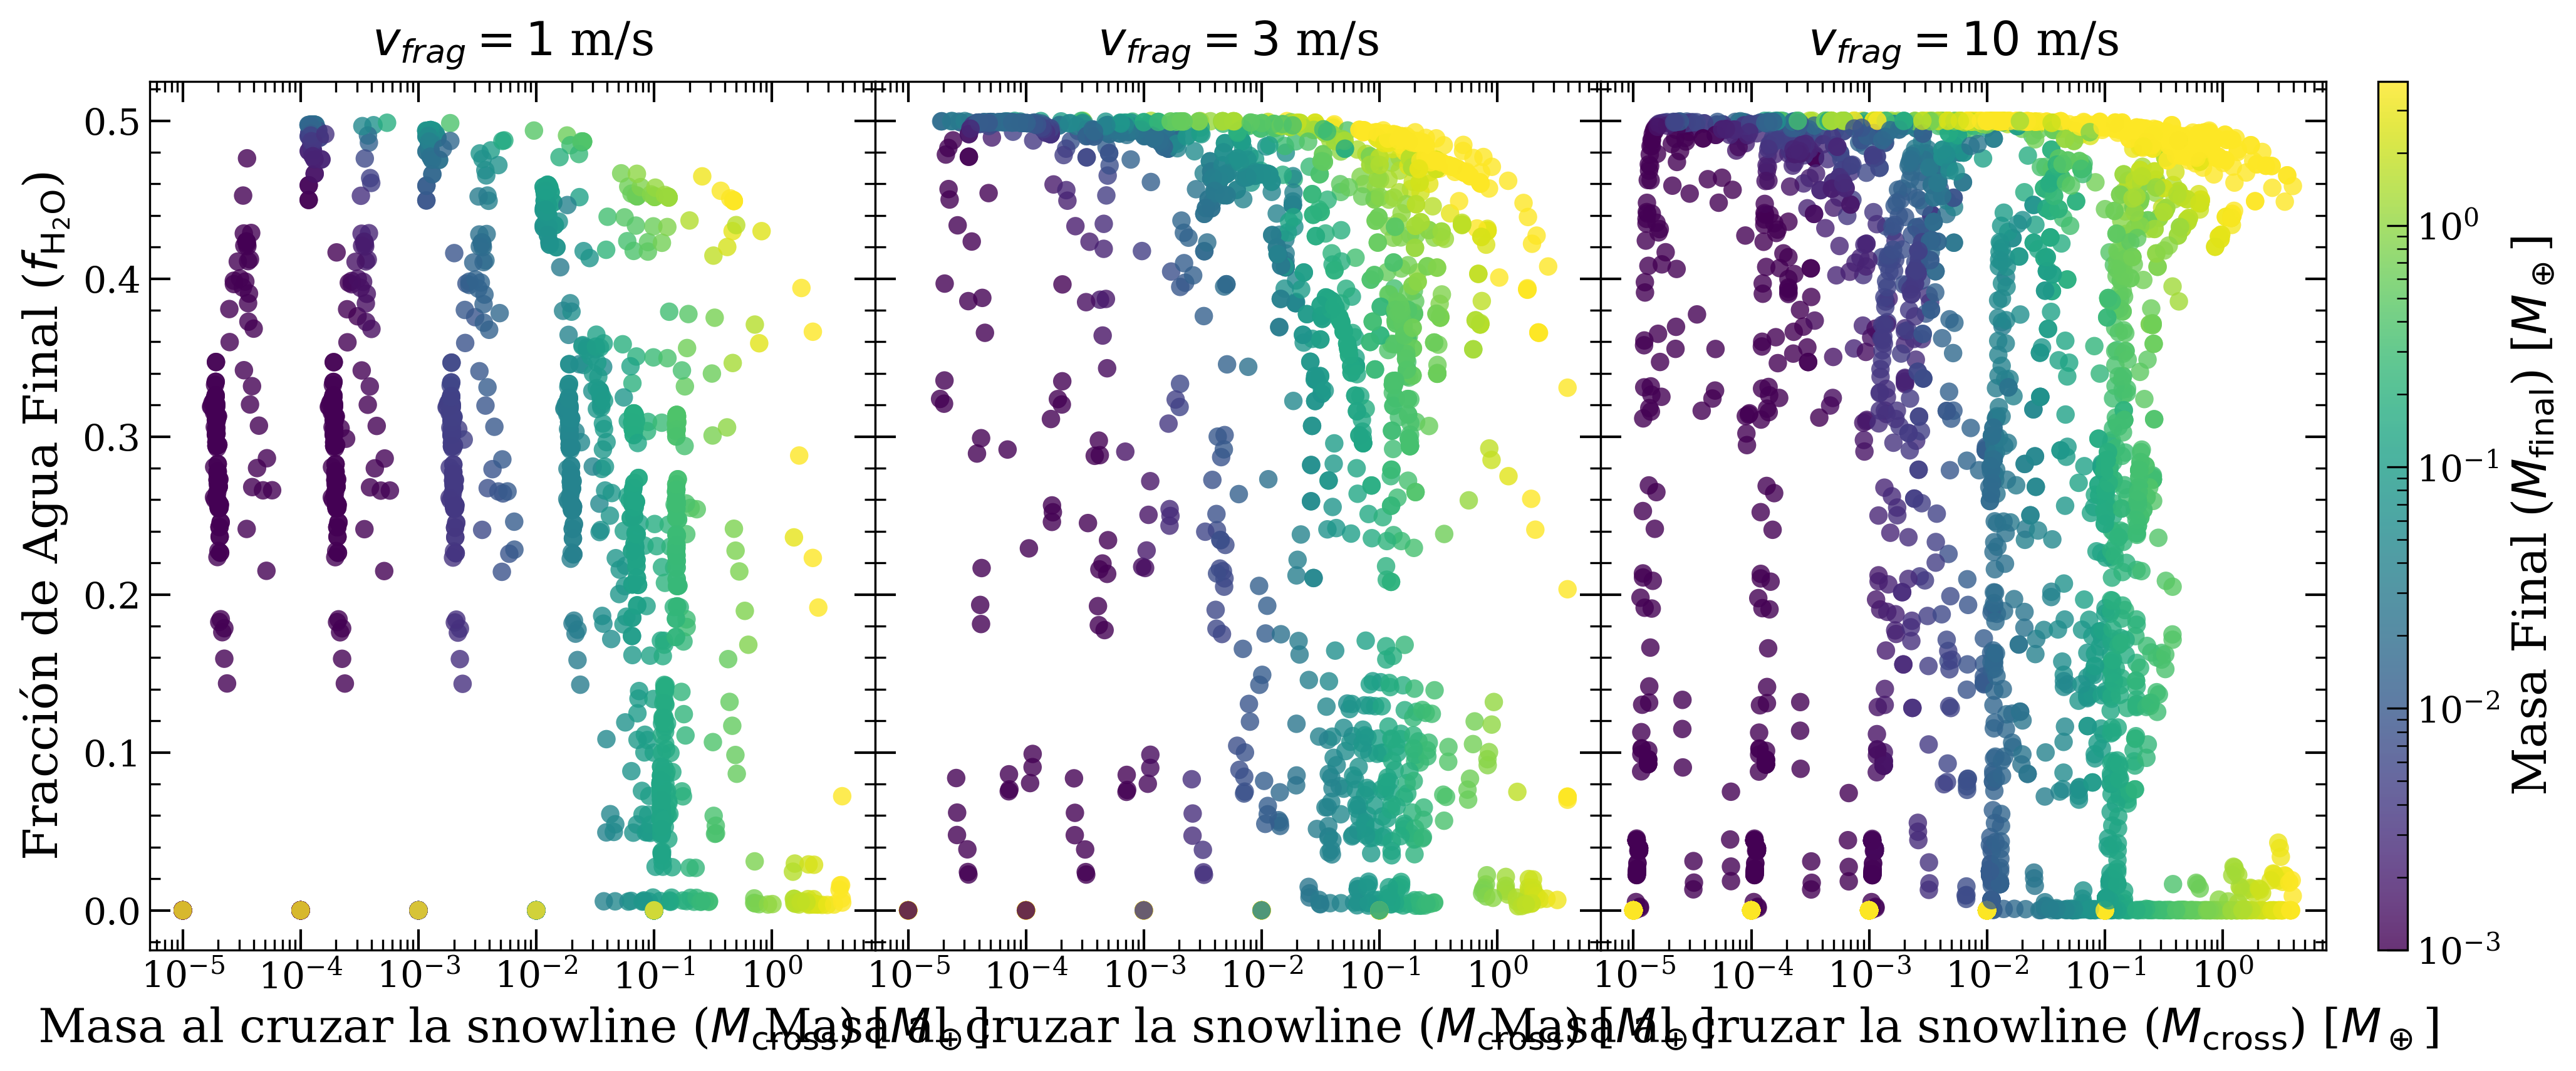
\includegraphics[width=0.49\textwidth]{figures/apendice/FigD_Mcross.png}
    \caption{\textit{Izquierda:} Masa final $M_c$ en función de $M_{\rm cross}$
    para distintas configuraciones de gap.
    \textit{Derecha:} Fracción de agua $f_{\rm H_2O}$ en función de $M_{\rm cross}$.
    La dispersión en ambas variables es menor al 5\% para el rango de
    $M_{\rm cross}$ explorado, validando la robustez numérica de los resultados.}
    \label{fig:ap_mcross_masa}
    \label{fig:ap_mcross_h2o}
\end{figure}
